\documentclass{sn-article}

\title{Supplementary Information: Lunar Crustal Magnetic Field Heterogeneity and Implications for Biological Systems at Candidate Landing Sites}
\author[1]{Richard Barker}
\author[2]{Co-Authors}
\affil[1]{Space Life Sciences, University of Wisconsin-Madison, Madison, WI, USA}
\affil[2]{Astrobiology & Lunar Exploration Working Group}
\date{\today}

\begin{document}
\maketitle

\section*{Extended Methods}

\subsection*{Bilinear Interpolation and Polar Baseline Integration}
The crustal magnetic field data sourced from \citet{Hood2020} and \citet{Hood2022} are derived from Lunar Prospector and SELENE (Kaguya) magnetometer observations at an equivalent altitude of \SI{30}{\kilo\meter}. For mid-latitude sites ($\le \SI{65}{\degree}|\text{lat}|$), bilinear interpolation was performed across the 2D gridded components $(B_r, B_\theta, B_\phi)$. For South Polar candidate landing sites ($\SI{84}{\degree}\text{S}$ to $\SI{90}{\degree}\text{S}$) and Chandrayaan-3 ($\SI{69.37}{\degree}\text{S}$), baseline vector and total field values were integrated from the South Polar spherical harmonic and equivalent source dipole models of \citet{Hood2022} and \citet{Tsunakawa2015}.

\subsection*{Coordinate Database Compilation}
Landing site coordinates were compiled from official NASA Artemis III Candidate Landing Regions reports \citep{NASA2022}, Lunar Reconnaissance Orbiter Camera (LROC) surface coordinates for Apollo 11--17, and published landing site telemetry for Chang'e 3, 4, 5, and Chandrayaan-3.

\section*{Supplementary Figures}

\begin{figure}[h]
\centering
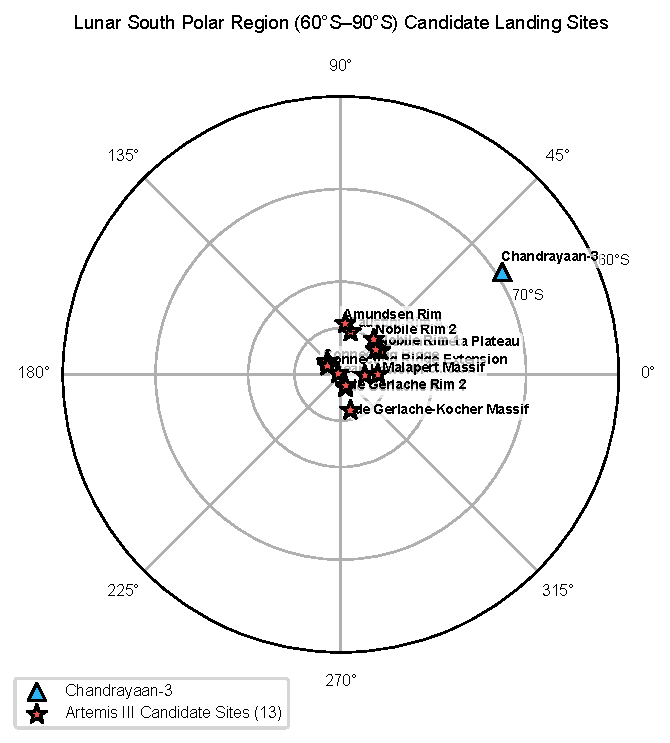
\includegraphics[width=\columnwidth]{../figures/fig_S1_polar_detail.pdf}
\caption{\textbf{Supplementary Figure S1: Lunar South Polar region ($\SI{60}{\degree}\text{S}$ to $\SI{90}{\degree}\text{S}$) candidate landing sites.} Polar stereographic projection displaying the 13 Artemis III candidate landing regions (red stars) and Chandrayaan-3 (blue triangle) in relation to South Polar latitude rings.}
\label{fig:S1_polar_detail}
\end{figure}

\begin{figure}[h]
\centering
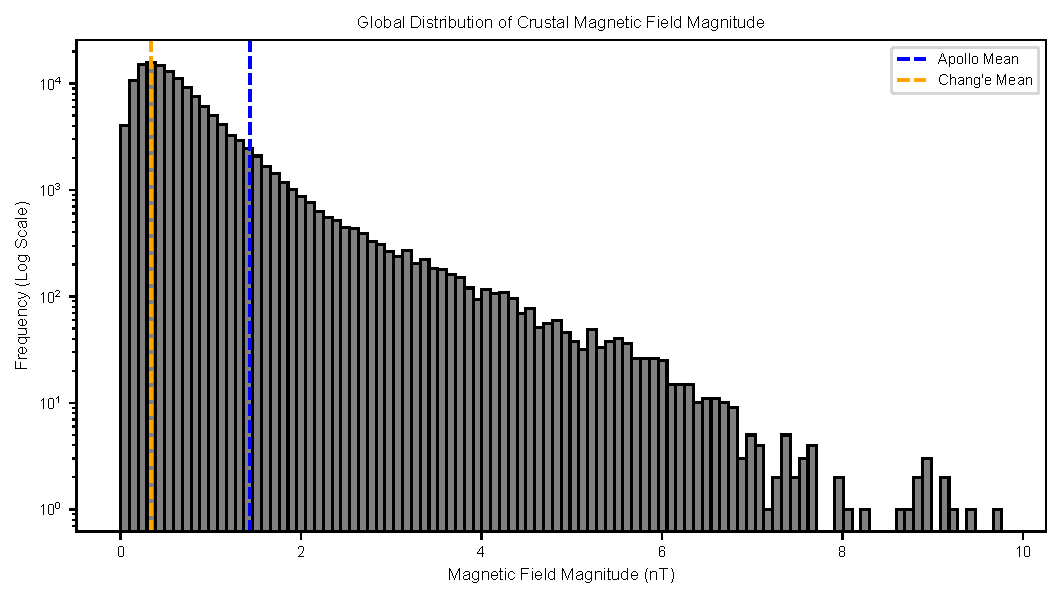
\includegraphics[width=\columnwidth]{../figures/fig_S2_field_histogram.pdf}
\caption{\textbf{Supplementary Figure S2: Global distribution of lunar crustal magnetic field magnitude.} Histogram showing the frequency distribution of $|\mathbf{B}|$ at \SI{30}{\kilo\meter} across 140,940 grid points, with global median (\SI{0.56}{\nano\tesla}), global mean (\SI{0.77}{\nano\tesla}), Artemis III candidate site mean (\SI{0.59}{\nano\tesla}), Apollo 16 (\SI{4.94}{\nano\tesla}), and Chang'e 4 (\SI{0.72}{\nano\tesla}) highlighted.}
\label{fig:S2_field_histogram}
\end{figure}

\section*{Data and Code Availability}
The full machine-readable landing site database, processed global grids, figure generation scripts, and interactive WebGL globe source code are available in the public GitHub repository (\url{https://github.com/dr-richard-barker/lunar-magnetic-biology}) and archived under DOI: 10.5281/zenodo.XXXXXXX.

\bibliographystyle{unsrtnat}
\bibliography{references}

\end{document}
